\begin{wrapfigure}{R}{0.37\linewidth}
%% \small
%% \begin{minipage}[t]{0.65\linewidth}
%%   \mytitle{interaction semantics}\\
%% $
%%   %% \begin{stackTL}
%%   %%   state \triangleq (\Memory, \overrightarrow{(\msem, \msem.\texttt{state})}) \\
%%   %%   (\istt, \mem) \iestep{e} (\istt', \mem') \defeq \\
%%   %%   \begin{array}{l@{\;}l@{\;}l}
%%   %%     & \caselabel{STEP} & \forall \msem, \tl, e, \mem, \stt, \mem', \stt',~ (\mem, \stt) \estep{e} (\mem', \stt') \implies (\mem, ((\msem, \stt) \cons \tl)) \iestep{e} (\mem', (\msem, \stt') \cons \tl) \\
%%   %%     & \caselabel{CALL} & \forall \msem, \msem', \tl, \mem, \mem', \stt_{\msem}, \args, \stt_{\msem'},~
%%   %%       \msem.\texttt{at\_external} \; (\mem, \stt) \; \args \land \msem'.\texttt{init\_core} \; \args \; (\mem', \stt') \implies \\
%%   %%     & & (\mem, (\msem, \stt) \cons \tl) \iestep{e} (\mem', (\msem', \stt') \cons (\msem, \stt) \cons \tl) \\
%%   %%     & \caselabel{RET} & \forall \msem, \msem', \tl, \mem, \mem', \stt_{\msem}, \args, \stt_{\msem'},~
%%   %%       \msem.\texttt{halted} \; (\mem, \stt) \; \retv \land \msem'.\texttt{after\_external} \; \stt' \; \retv \; (\mem', \stt'') \implies \\
%%   %%     & & (\mem, (\msem, \stt) \cons (\msem', \stt') \cons \tl) \iestep{e} (\mem', (\msem', \stt'') \cons \tl) \\
%%   %%   \end{array}
%%   %% \end{stackTL}
%%   \begin{stackTL}
%%     %% \textrm{State} \defeq (\Memory, \overrightarrow{(\msem, \States{\msem})}) \\
%%     %% \textrm{State} \defeq \Memory \times \overrightarrow{\Msem \times \States{\Msem}} \\
%%     \textrm{State} \defeq \{ (\mem, \overrightarrow{(\msem, \stt)} \; | \; \mem \in \Memory \land \msem \in \Msem \land \stt \in \msem.\texttt{state} \} \\
%%     \Genv \defeq \{ \genv \; | \; \genv \in \overrightarrow{\Msem} \} \\
%%     \genv.\texttt{lookup\_modsem}(f) \defeq \{ \msem \; | \; \msem \in \genv \land f \in \textrm{ftns}(\msem.\texttt{senv}) \} \\
%%     \begin{array}{l@{\;}l@{\;}l}
%%       & \caselabel{STEP} & \genv \models (\mem, ((\msem, \stt) \cons \tl)) \iestep{e} (\mem', (\msem, \stt') \cons \tl) \myif \\
%%       & & (\mem, \stt) \estep{e} (\mem', \stt') \\
%%       & \caselabel{CALL} & \genv \models (\mem, (\msem, \stt) \cons \tl) \iestep{e} (\mem', (\msem', \stt') \cons (\msem, \stt) \cons \tl) \myif \\
%%       & & \exists \args,~ \msem.\texttt{at\_external}(\mem, \stt) = \some{\args} \land \msem' \in \genv.\texttt{lookup\_modsem}(c.\texttt{f}) \; \land \\
%%       & & (\mem', \stt') \in \msem'.\texttt{init\_core}(\args) \\
%%       & \caselabel{RET}  & \genv \models (\mem, (\msem, \stt) \cons (\msem', \stt') \cons \tl) \iestep{e} (\mem', (\msem', \stt'') \cons \tl) \myif \\
%%       & & \exists \retv,~ \msem.\texttt{halted}(\mem, \stt) = \some{\retv} \; \land \\
%%       & & \msem'.\texttt{after\_external}(\stt',\retv) = \some{(\mem', \stt'')} \\
%%     \end{array}
%%     %% \genv \models (\istt, \mem) \iestep{e} (\istt', \mem') \defeq \\
%%     %% \begin{array}{l@{\;}l@{\;}l}
%%     %%   & \caselabel{STEP} & \forall \msem, \tl, e, \mem, \stt, \mem', \stt',~ (\mem, \stt) \estep{e} (\mem', \stt') \implies \\
%%     %%   & & (\mem, ((\msem, \stt) \cons \tl)) \iestep{e} (\mem', (\msem, \stt') \cons \tl) \\
%%     %%   & \caselabel{CALL} & \forall \msem, \msem', \tl, \mem, \mem', \stt, \stt', \args,~ \\
%%     %%   & & \msem.\texttt{at\_external} \; (\mem, \stt) \; \args \land
%%     %%       \msem' \in \genv.\texttt{lookup\_modsem}(c.\texttt{f}) \; \land \\
%%     %%   & & \msem'.\texttt{init\_core} \; \args \; (\mem', \stt') \implies \\
%%     %%   & & (\mem, (\msem, \stt) \cons \tl) \iestep{e} (\mem', (\msem', \stt') \cons (\msem, \stt) \cons \tl) \\
%%     %%   & \caselabel{RET} & \forall \msem, \msem', \tl, \mem, \mem', \stt_{\msem}, \args, \stt_{\msem'},~ \\
%%     %%   & & \msem.\texttt{halted} \; (\mem, \stt) \; \retv \land \msem'.\texttt{after\_external} \; \stt' \; \retv \; (\mem', \stt'') \implies \\
%%     %%   & & (\mem, (\msem, \stt) \cons (\msem', \stt') \cons \tl) \iestep{e} (\mem', (\msem', \stt'') \cons \tl) \\
%%     %% \end{array}
%%   \end{stackTL}
%% $
%% \end{minipage}%
\mytitle{loading process}\\
%% \centering
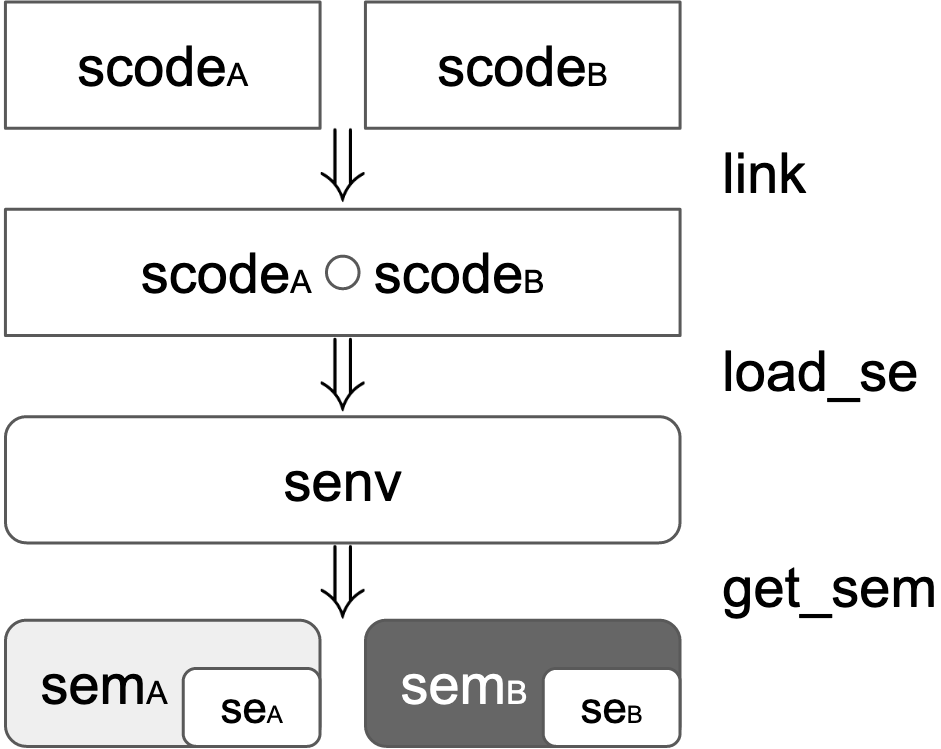
\includegraphics[width=1\linewidth]{fig-load.png}
%% \caption{Loading Process}
%% \label{fig:load}

%% \begin{minipage}{0.5\linewidth}
%% \begin{figure}
%%   \centering
%%   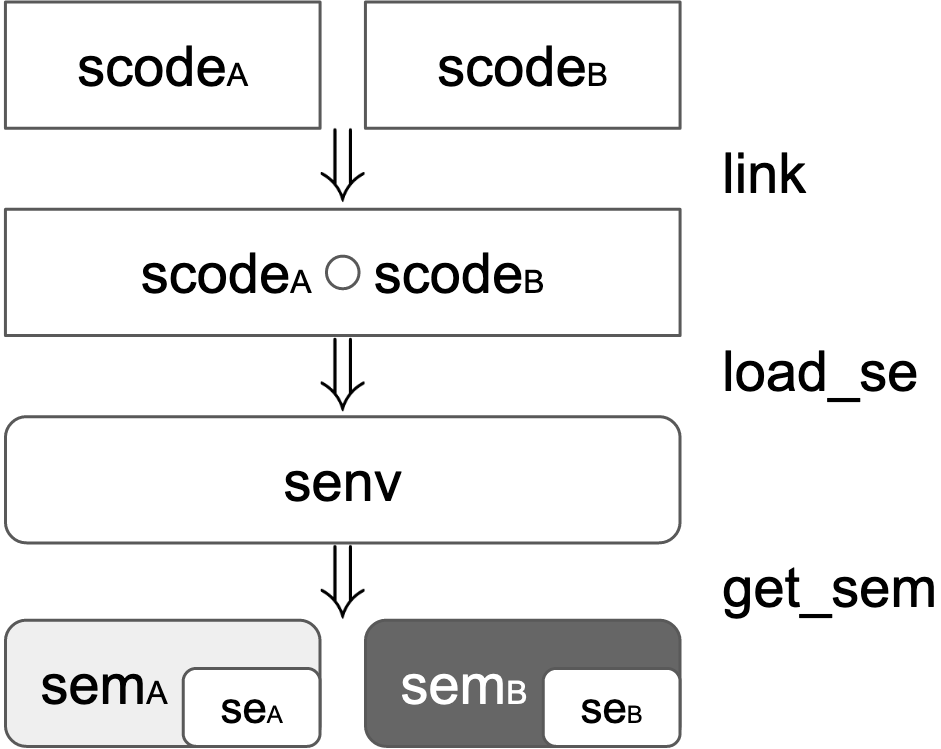
\includegraphics[width=0.25\linewidth]{fig-load.png}
%%   \caption{Loading Process}
%%   \label{fig:load}
%% \end{figure}
%% \end{minipage}

%% \begin{subfigure}{.4\linewidth}
%%   \centering
%%   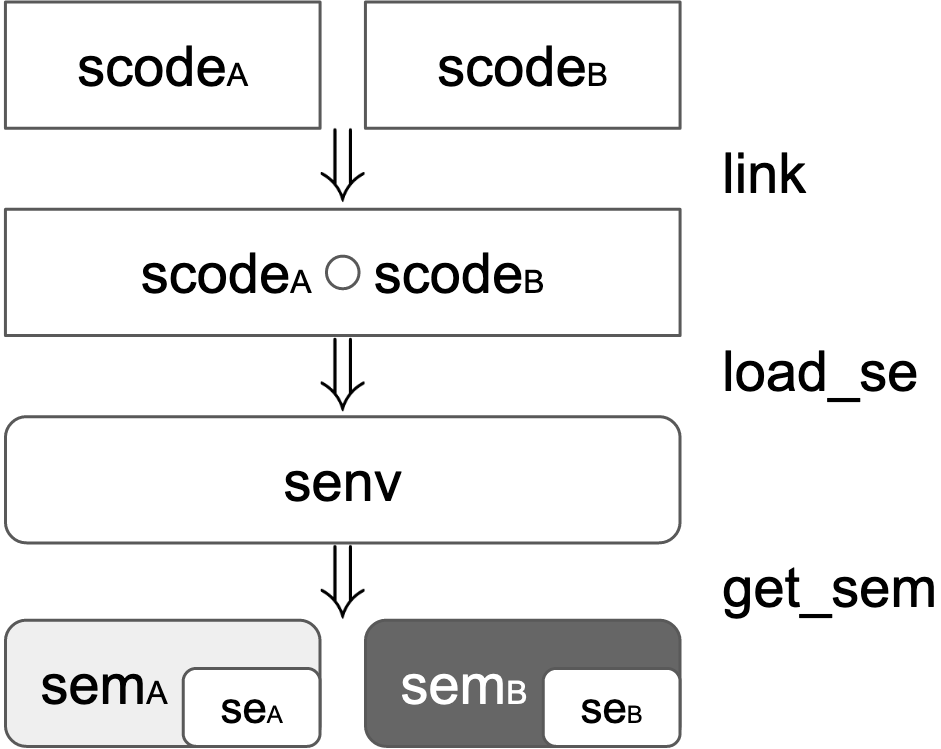
\includegraphics[width=0.25\linewidth]{fig-load.png}
%%   \caption{Loading Process}
%%   \label{fig:load}
%% \end{subfigure}

%% \youngju{lookup\_modsem is actually deterministic (loading process guarantees it)}

%% \youngju{Maybe we can use ``bar'' notation like princeton did}
\caption{Loading in Interaction Semantics}
\label{fig:full-sem}
\vspace*{-2mm}
\end{wrapfigure}

